\documentclass[10pt,a4paper]{article}

\usepackage[top=2.0cm,bottom=2.2cm,left=2.2cm,right=2.2cm]{geometry}
\usepackage[T1]{fontenc}
\usepackage{lmodern}
\usepackage{microtype}
\usepackage{booktabs}
\usepackage{pgfplots}
\pgfplotsset{compat=1.18}
\usepackage{tikz}
\usepackage{xcolor}
\usepackage{parskip}
\usepackage{titlesec}
\usepackage[hidelinks]{hyperref}
\usepackage{caption}
\usepackage{fancyhdr}
\usepackage{lastpage}
\usepackage{setspace}
\setlength{\headheight}{20pt}
\addtolength{\topmargin}{-8pt}

%% Colours
\definecolor{uoeblue}{RGB}{0,60,113}
\definecolor{lightgray}{RGB}{248,248,248}
\definecolor{midgray}{RGB}{130,130,130}
\definecolor{darkgray}{RGB}{70,70,70}

%% Section style
\titleformat{\section}
  {\normalfont\large\bfseries\color{uoeblue}}
  {}
  {0em}
  {}
  [\vspace{-3pt}{\color{uoeblue}\rule{\linewidth}{0.6pt}}]
\titlespacing*{\section}{0pt}{9pt}{4pt}

%% Caption style
\captionsetup{font=small, labelfont=bf, skip=3pt}

%% Paragraph spacing
\setlength{\parindent}{0pt}
\setlength{\parskip}{4.5pt}

%% Header / footer
\pagestyle{fancy}
\fancyhf{}
\lhead{\small\textcolor{darkgray}{InfraQ \textemdash\ ACP CW3}}
\rhead{\small\textcolor{darkgray}{University of Edinburgh, School of Informatics}}
\cfoot{\small\textcolor{midgray}{\thepage\,/\,\pageref{LastPage}}}
\renewcommand{\headrulewidth}{0.3pt}
\renewcommand{\headrule}{\hbox to\headwidth{\color{midgray}\leaders\hrule height \headrulewidth\hfill}}

\begin{document}

%% ─── Title ──────────────────────────────────────────────────────────────────
\vspace*{-0.3em}
\begin{center}
  {\LARGE\bfseries\color{uoeblue}InfraQ}\\[5pt]
  {\large A Scheduling Gateway for Shared Local LLM Inference}\\[6pt]
  {\small Advanced Cloud Programming\;\textbullet\;
   CW3\;\textbullet\;
   University of Edinburgh\;\textbullet\;
   April 2026}
\end{center}
{\color{uoeblue}\rule{\linewidth}{1.0pt}}
\vspace{3pt}

\textit{InfraQ implements four LLM request scheduling strategies on top of RabbitMQ, Redis,
PostgreSQL, and a Python asyncio worker, running on Mac~M1 without CUDA.
A built-in benchmark framework measures each strategy under controlled workloads.
Across 45 runs of 100-request workloads, cache-aware dispatching on repeated prompts
achieved \textbf{5.6$\times$ higher throughput} and \textbf{76\% lower average latency}
compared to non-cached strategies.}

\vspace{2pt}

%% ─── 1. Problem and Idea ────────────────────────────────────────────────────
\section{Problem and Idea}

Teams running a shared Ollama instance face three problems: concurrent requests pile up
with no queue, repeated prompts get re-inferred every time, and there is no way to measure
whether a different scheduling approach would help. vLLM and SGLang solve this at the
GPU kernel level, but both require NVIDIA hardware most small teams cannot justify.
LiteLLM proxies requests; it does not schedule them.

InfraQ moves continuous batching%
\footnote{Kwon et al., \textit{Efficient Memory Management for LLM Serving with
PagedAttention}, SOSP~2023.}
and prefix caching%
\footnote{Zheng et al., \textit{SGLang: Efficient Execution of Structured Language Model
Programs}, NeurIPS~2024.}
from the GPU layer to the infrastructure layer, approximated with RabbitMQ slot management
and a Redis text cache.
More importantly, InfraQ is a \textbf{research platform}: switching strategies requires
changing one Redis key, and a benchmark framework controls the full experiment
lifecycle---idle confirmation, strategy application, cache clearing, request
submission---producing results comparable across strategies on identical workloads.

%% ─── 2. Scheduling Strategies ───────────────────────────────────────────────
\section{Scheduling Strategies}

\textbf{Sequential} processes one request at a time. No concurrency. It is the
performance floor.

\textbf{Static batching} collects $N$ requests, fires them all at once, then waits for
the entire batch before accepting more. The slowest request holds every completed slot
idle---a structural source of tail latency.

\textbf{Continuous dispatching} (after vLLM) maintains $K$ concurrent slots via an
asyncio semaphore. Any slot that completes immediately admits the next request, eliminating
batch-boundary stalls. Ollama receives $K$ simultaneous HTTP connections and, with
\texttt{OLLAMA\_NUM\_PARALLEL} set accordingly, merges them into a single tensor forward
pass---InfraQ manages the slot lifecycle; Ollama handles batched inference.

\textbf{Cache-aware dispatching} (after SGLang) adds a Redis lookup before any slot
is acquired. The cache key is the SHA-256 hash of model name and prompt text. Hits return
in ${\sim}$11\,ms without touching Ollama; misses proceed through continuous dispatching
and write their result to Redis (TTL: 1~hour). This approximates KV-cache reuse at the
infrastructure layer without shared GPU memory.

The worker writes its runtime state to Redis every second. When the desired configuration
changes, the worker drains all in-flight tasks and restarts under the new strategy without
container restarts, enabling clean back-to-back experiments.

%% ─── 3. Architecture ────────────────────────────────────────────────────────
\section{Architecture}

The gateway (Spring Boot) returns 202 immediately on every request, writing to PostgreSQL,
Redis, and RabbitMQ in sequence. The worker (Python asyncio) consumes from RabbitMQ and
applies the active scheduling strategy. Ollama runs natively on the host, accessed via
\texttt{host.docker.internal}---Mac Metal GPU acceleration requires no passthrough.

\begin{center}
\begin{tikzpicture}[
  box/.style={draw=uoeblue!55, rounded corners=3pt,
    minimum width=1.85cm, minimum height=0.62cm,
    font=\small, fill=uoeblue!8},
  hbox/.style={draw=uoeblue, rounded corners=3pt,
    minimum width=1.85cm, minimum height=0.62cm,
    font=\small\bfseries, fill=uoeblue!22},
  arr/.style={->, >=stealth, thick, color=darkgray},
  lbl/.style={font=\scriptsize\itshape, color=darkgray},
  every node/.style={align=center}
]
  \node[hbox] (cli) at (0,0)     {Browser};
  \node[box]  (gw)  at (2.85,0)  {Gateway\\(Spring Boot)};
  \node[box]  (mq)  at (5.7,0)   {RabbitMQ};
  \node[box]  (wk)  at (8.55,0)  {Worker\\(asyncio)};
  \node[hbox] (ol)  at (8.55,-1.65) {Ollama\\(Metal GPU)};
  \node[box]  (rd)  at (5.7,-1.65)  {Redis};
  \node[box]  (pg)  at (2.85,-1.65) {PostgreSQL};

  \draw[arr] (cli) -- (gw) node[lbl,above,midway]{POST};
  \draw[arr] (gw)  -- (mq) node[lbl,above,midway]{enqueue};
  \draw[arr] (mq)  -- (wk) node[lbl,above,midway]{consume};
  \draw[arr] (wk)  -- (ol) node[lbl,right,midway]{infer};
  \draw[arr] (wk)  -- (rd) node[lbl,above,midway]{result};
  \draw[arr] (rd)  -- (gw) node[lbl,above,midway]{status/cache};
  \draw[arr] (gw)  -- (pg) node[lbl,right,midway]{persist};
  \draw[->, >=stealth, thick, dashed, color=uoeblue!60]
    (rd) to[bend right=18] node[lbl,below,midway]{config} (wk);
\end{tikzpicture}
\end{center}
\vspace{-2pt}

Redis serves four roles: request status fast-path for browser polling ($<$1\,ms);
prompt text cache; real-time atomic metric counters; and the configuration channel
between gateway and worker (dashed). PostgreSQL stores permanent records---request
histories, per-request timing, and benchmark run statistics that outlast Redis TTLs.

%% ─── 4. Results ─────────────────────────────────────────────────────────────
\section{Experimental Results}

All experiments: MacBook Air M1 8\,GB, Qwen2.5:1.5b via Ollama, 100~requests per run,
5~repeats per condition. Data: \texttt{summary.csv} and \texttt{manifest.json} in submission.

\begin{table}[h]
\centering
\caption{Experiment A --- unique prompts (no cache benefit). 5-run averages.}
\small\setlength{\tabcolsep}{7pt}
\begin{tabular}{lcrrr}
\toprule
Strategy        & Slots & Avg latency & P95       & Throughput   \\
\midrule
Sequential      & 1     & 188\,s      & 442\,s    & 0.213\,req/s \\
Static batching & 8     & 185\,s      & 438\,s    & 0.213\,req/s \\
Continuous      & 8     & 180\,s      & \textbf{426\,s} & \textbf{0.219\,req/s} \\
Cached          & 8     & 179\,s      & 430\,s    & 0.218\,req/s \\
\bottomrule
\end{tabular}
\end{table}

\vspace{-4pt}

\begin{table}[h]
\centering
\caption{Experiment B --- repeated prompts (hot prompt set). 5-run averages.}
\small\setlength{\tabcolsep}{6pt}
\begin{tabular}{lcrrrr}
\toprule
Strategy          & Slots & Avg latency & P95     & Throughput            & Hit rate \\
\midrule
Sequential        & 1     & 311\,s      & 584\,s  & 0.165\,req/s          & 0\%      \\
Static batching   & 4     & 298\,s      & 557\,s  & 0.173\,req/s          & 0\%      \\
Continuous        & 4     & 299\,s      & 565\,s  & 0.170\,req/s          & 0\%      \\
\bfseries Cached  & \bfseries 4 & \bfseries 73\,s & \bfseries 96\,s &
\bfseries 0.961\,req/s & \bfseries 71\% \\
\bottomrule
\end{tabular}
\end{table}

\vspace{-2pt}

\begin{figure}[h]
\centering
\begin{tikzpicture}
\begin{axis}[
  xbar,
  width=0.78\linewidth,
  height=4.6cm,
  xmin=0, xmax=1.12,
  xlabel={Throughput (req/s)},
  ytick={0,1,2,3},
  yticklabels={Sequential 1sl, Static 4sl, Continuous 4sl, Cached 4sl},
  ymin=-0.6, ymax=3.6,
  nodes near coords,
  nodes near coords align={horizontal},
  every node near coord/.style={font=\small},
  bar width=9.5pt,
  tick label style={font=\small},
  xlabel style={font=\small},
  title={Throughput on repeated-prompt workload (Experiment B)},
  title style={font=\small\bfseries, color=darkgray},
  xmajorgrids=true,
  grid style={dashed, gray!25},
  axis line style={midgray},
  tick style={midgray},
]
\addplot[fill=uoeblue!70, draw=uoeblue!90] coordinates {
  (0.165,0) (0.173,1) (0.170,2) (0.961,3)
};
\end{axis}
\end{tikzpicture}
\caption{Cache-aware dispatching (71\% hit rate) achieves 5.6$\times$ higher throughput on repeated prompts.
Non-cached strategies are bound by Ollama's total token generation rate.}
\end{figure}

On \textbf{unique prompts}, scheduling gains are modest. Continuous dispatching reduces
P95 latency by 12\,s versus static batching (426\,s vs.\ 438\,s), consistent with
eliminating the wait-for-slowest-in-batch effect. Total token generation rate is the
bottleneck; concurrency alone cannot exceed it.

On \textbf{repeated prompts}, caching is the dominant lever. At 71\% hit rate,
cache-aware dispatching delivers 5.6$\times$ higher throughput and 76\% lower average
latency (73\,s vs.\ 299\,s). Cache hits bypass Ollama entirely; P95 falls from
${\sim}$565\,s to 96\,s.

\textbf{Slot-count ablation (cached strategy, repeated workload):} 4~slots
(0.961\,req/s, 71\% hit rate) outperforms 8~slots (0.699\,req/s, 67\% hit rate).
More slots produce more simultaneous cache misses before warmup, reducing hit rate and
increasing Ollama contention simultaneously. The optimal slot count for cache-aware
dispatching is not ``as many as possible.''

%% ─── 5. Completeness ────────────────────────────────────────────────────────
\section{Completeness}

All four strategies are fully implemented and hot-switchable on a running system.
The benchmark framework runs automatically across a 45-run matrix (100~requests per run,
5~repeats per condition). A web interface provides a chat tab, a real-time metrics
dashboard, and benchmark history with per-run comparison charts. The system starts with
\texttt{docker compose up}; Ollama and the Qwen2.5:1.5b model are the only external
dependencies.

%% ─── 6. AI Usage ────────────────────────────────────────────────────────────
\section{AI Usage}

Claude Code (Anthropic) assisted with Spring Boot boilerplate, Python asyncio control
flow, and system design discussion. Strategy definitions, experimental methodology, and
result analysis are the author's own work. All AI-generated code was tested and debugged
locally before submission.

\end{document}
